\documentclass[12pt,aspectratio=43,dvipsnames,table]{beamer}
\usepackage[french]{babel}
\usepackage[T1]{fontenc}
\usepackage[utf8]{inputenc}
\usepackage{url}
\usepackage{multirow}
\usepackage{mathtools}
% \usepackage{color}

\usetheme{default}
\useinnertheme{default}
\useoutertheme{default}
\usefonttheme{serif}
\usecolortheme[named=WildStrawberry]{structure}

% Marges autour des slides
\setbeamersize{text margin left=5mm, text margin right=5mm}

% Suppression des symboles de navigation
\beamertemplatenavigationsymbolsempty

% Définition du pied de page
\setbeamertemplate{footline} {
  \hfill{
    \insertshortdate ~- %
    page \insertframenumber~sur~\inserttotalframenumber %
    %\hspace*{0.1cm}
  } \vspace*{0.05cm}
}

% Définition des espacements des listes
\setlength{\leftmargini}{0.6cm}
\setlength{\leftmarginii}{0.4cm}
\setlength{\leftmarginiii}{0.4cm}

\title{Recherche d'information cross-lingue}
\subtitle{Applications multilingues - module X9IT100}
\author{Florian Boudin}
\institute{Département informatique, Université de Nantes}
\date[30 juillet 2013 / Rév.~1]{Révision~1 du 30 juillet 2012}

\begin{document}


%-B--------------------------------------------------------------------------B-%
\frame[plain]{\titlepage}
%-E--------------------------------------------------------------------------E-%


%##############################################################################%
\section{Introduction}
%##############################################################################%


%-B--------------------------------------------------------------------------B-%
\begin{frame}
    \frametitle{Préface}
    \begin{itemize} \itemsep10pt
        \item Volume horaire (2h40)
        \item Notions abordées dans ce cours
        \begin{itemize}
            \item Rappels des notions de RI
            \item Les difficultés liées aux langues
            \item ...
        \end{itemize}
        \item Ce cours est basé sur le livre \textit{Cross-Language Information 
              Retrieval} de Jian-Yun Nie~\cite{DBLP:series/synthesis/2010Nie}.
    \end{itemize}
\end{frame}
%-E--------------------------------------------------------------------------E-%


%-B--------------------------------------------------------------------------B-%
\begin{frame}
    \frametitle{Introduction}
    \begin{itemize} \itemsep10pt
        \item La \textbf{Recherche d'Information} (RI) fait partie intégrante de
              notre vie quotidienne.
        \item Dans la plupart des cas, nous recherchons des documents rédigés 
              dans notre langue maternelle, en général celle utilisée dans la 
              requête.
        \item \textbf{Cependant...}
        \begin{itemize}
            \item L'information pertinente n'est pas toujours disponible dans 
                  notre langue maternelle.
            \item Le web offre une mine d'information riche et multilingue à 
                  laquelle nous souhaitons avoir accès.
        \end{itemize}
        \item \'Emergence de la problématique de la RI cross-lingue
    \end{itemize}
\end{frame}
%-E--------------------------------------------------------------------------E-%


%##############################################################################%
\section{Rappels des notions de RI}
%##############################################################################%


%-B------------------------------PLAN----------------------------------------B-%
\begin{frame}
\frametitle{Plan}
\tableofcontents[sectionstyle=show,subsectionstyle=hide,subsubsectionstyle=hide]
\end{frame}
%-E--------------------------------------------------------------------------E-%


%-B--------------------------------------------------------------------------B-%
\begin{frame}
    \frametitle{Le processus de recherche d'information}
    \begin{figure}
    \centering
    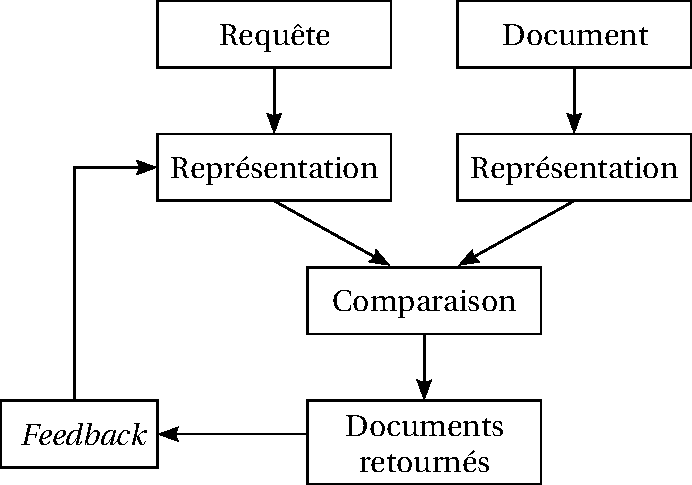
\includegraphics[width=0.75\textwidth]{img/typicalIR.pdf}
    \caption{Processus de recherche d'information (Figure 1.1 
             de~\cite{DBLP:series/synthesis/2010Nie}).}
    \end{figure}
\end{frame}
%-E--------------------------------------------------------------------------E-%


%-B--------------------------------------------------------------------------B-%
\begin{frame}[allowframebreaks]
    \frametitle{Modèles de RI}
    \begin{itemize} \itemsep10pt
        \item Un modèle définit la représentation des documents et des requêtes 
              ainsi que la fonction de pondération.
        \item La plupart des modèles sont construits sur la notion de 
              \textit{terme}, qui peut être un mot (e.g.~\textit{computer}), un 
              stem (e.g.~\textit{comput}) ou une expression multimots 
              (e.g.~\textit{computer system}).
        \item \textbf{Modèle booléen}
        \begin{itemize}
            \item Les documents sont représentés par une conjonction de termes, 
                  e.g.~$D = t_1 \land t_2 \land t_3$ qui signifie que les termes
                  $t_1$, $t_2$ et $t_3$ apparaissent dans $D$.
            \item Une requête est représentée par une expression booléenne, 
                  e.g.~$Q = (t_1 \land t_2) \lor t_3$.
            \item Un document est considéré comme pertinent si et seulement si 
                  il y a l'implication logique $D \to P$.
        \end{itemize}

        \framebreak

        \item \textbf{Modèle vectoriel}~\cite{DBLP:journals/cacm/SaltonWY75,DBLP:books/mg/SaltonG83}
        \begin{itemize}
            \item Les documents et requêtes sont représentés par des vecteurs 
                  dans un espace vectoriel composé de tous les termes.
            \item Dans chaque vecteur, chaque élément ($d_i$ ou $q_i$, 
                  $1 \leq i \leq n$) représente le poids du terme.
        \end{itemize}
        %
        \vspace*{-0.5em}
        \begin{align*}
          \text{espace vectoriel~:} &~(t_1, t_2, \cdots, t_n) \\
          \text{document~:} &~(d_1, d_2, \cdots, d_n) \\
          \text{requête~:} &~(q_1, q_2, \cdots, q_n)
        \end{align*}
        \vspace*{-1.5em}
        %
        \begin{itemize}
            \item Les poids des termes peuvent être binaires, i.e.~1 pour la 
                  présence et 0 l'absence, ou calculés avec $tf \times idf$.
            \item La pertinence des documents est habituellement calculée avec 
                  une mesure de similarité cosinus.
        \end{itemize}

        \framebreak

        \item \textbf{Modèle probabiliste}~\cite{robertson1976relevance}
         \begin{itemize}
            \item Le score de pertinence d'un document $D$ par rapport à une 
                  requête $Q$ est estimé à partir de $P(\text{pertinence}|D,Q)$.
            \item Okapi BM25~\cite{DBLP:conf/trec/RobertsonWHGL92} est le modèle 
                  le plus utilisé.
            \begin{equation*}
              \text{score}(D,Q) = \sum_{i=1}^{n} \text{idf}(q_i) \cdot 
              \frac{f(q_i, D) \cdot (k_1 + 1)}
              {f(q_i, D) + k_1 \cdot (1 - b + b \cdot \frac{|D|}{\text{avgdl}})}
            \end{equation*}
            \item où $f(q_i, D)$ est la fréquence du terme $q_i$ dans $D$, 
                  $avgdl$ est la longueur moyenne des documents, 
                  $k_1 \in [1.2,2.0]$ et $b = 0.75$.
        \end{itemize}

        \framebreak

        \item \textbf{Modèle de langue}~\cite{DBLP:conf/sigir/PonteC98}
        \begin{itemize}
            \item Utiliser $P(D|Q)$ pour estimer le score de pertinence d'un 
                  document $D$ par rapport à une requête $Q$.
            \item Avec le théorème de Bayes, nous avons~:
            \begin{equation*}
              P(D|Q) = \frac{P(Q|D)P(D)}{P(Q)} \propto P(Q|D)P(D)
            \end{equation*}
            \item En considérant les termes de la requêtes comme indépendants~:
            \begin{equation*}
              P(Q|D) = \sum_{t_i \in Q} P(t_i | D)
            \end{equation*}
            \item $P(t_i | D)$ est estimée par un modèle de langue du document.
        \end{itemize}

    \end{itemize}
\end{frame}
%-E--------------------------------------------------------------------------E-%


%-B--------------------------------------------------------------------------B-%
\begin{frame}
    \frametitle{\'Evaluation}

    \begin{align*}
    \text{precision} & = \frac{\text{\# documents pertinents retrouvés}}
                              {\text{\# documents retrouvés}}
                              \\[1.5em]
    \text{rappel} & = \frac{\text{\# documents pertinents retrouvés}}
                           {\text{\# documents pertinents dans la collection}}
                           \\[1.5em]
    \text{MAP} & = \overbracket[1pt]{
                      \frac{1}{M} \sum_{j=1}^{M}
                   }^{\forall~\text{requêtes}} 
                   \underbracket[1pt]{
                    \Bigg( \frac{1}{N_j} \sum_{i=1}^{N_j} pr(d_{ij}) \Bigg)
                   }_{
                      \substack{
                        \text{moyenne des précisions} \\ 
                        \text{aux rangs des documents} \\ 
                        \text{pertinents}
                      }
                    }
    \end{align*}

\end{frame}
%-E--------------------------------------------------------------------------E-%


%##############################################################################%
\section{Les difficultés liées aux langues}
%##############################################################################%


%-B------------------------------PLAN----------------------------------------B-%
\begin{frame}
\frametitle{Plan}
\tableofcontents[sectionstyle=show,subsectionstyle=hide,subsubsectionstyle=hide]
\end{frame}
%-E--------------------------------------------------------------------------E-%

%-B--------------------------------------------------------------------------B-%
\begin{frame}
    \frametitle{Introduction}
    \begin{itemize} \itemsep10pt
      \item Les travaux en RI ont longtemps porté uniquement sur les langues 
            européennes.
      \item Cette situation a changée avec l'avènement du web et la 
            disponibilité de grandes collections de documents dans de nombreuses 
            langues.
      \item Bien que les traitements ``basiques'' développés pour les langues 
            européennes sont en partie ré-utilisable pour d'autres lanugues, 
            certaines nécessitent des traitements spécifiques.
    \end{itemize}
\end{frame}
%-E--------------------------------------------------------------------------E-%


%-B--------------------------------------------------------------------------B-%
\begin{frame}
    \frametitle{Langues Européennes}
    \begin{itemize} \itemsep10pt
      \item \textbf{Stemming} (racinisation)
      \begin{itemize}
        \item Porter~\cite{porter1980algorithm} et Krovetz~\cite{Krovetz:1993}
              pour l'anglais.
        \item Snowball\footnote{\url{http://snowball.tartarus.org/}}~: extension
              de l'algorithme de Porter à 15 langues.
        \item Les méthodes de stemming permettent souvent une amélioration de la
              performance mais pas toujours (les moteurs de recherche actuels 
              ne l'utilisent pas).
      \end{itemize}
      \item \textbf{Decompounding} (décomposition)
      \begin{itemize}
        \item Dans les langues agglutinantes (e.g.~Allemand, Néerlandais, 
              Finnois), les mots se forment à partir d'une racine lexicale à 
              laquelle on peut ajouter un certain nombre d'affixes.
        \item \textit{hungerstreiks} (de) est composé de \textit{hunger} (faim),
              \textit{strieks} (grève) et peut aussi s'écrire en deux mots 
              séparés.
      \end{itemize}


    

    \end{itemize}

\end{frame}
%-E--------------------------------------------------------------------------E-%


%-B--------------------------------------------------------------------------B-%
\begin{frame}
    \frametitle{}
\end{frame}
%-E--------------------------------------------------------------------------E-%


%##############################################################################%
\section{Références}
%##############################################################################%


%-B--------------------------------------------------------------------------B-%
\begin{frame}[allowframebreaks]
    \frametitle{References}
    \bibliographystyle{alpha}
    \bibliography{bibliography}
\end{frame}
%-E--------------------------------------------------------------------------E-%


\end{document}